\chapter{Find all groups}
The following problem will hopefully never be proposed at the IMO.
\begin{quote}
	Let $n$ be a positive integer and let $S = \left\{ 1,\dots,n \right\}$.
	Find all functions $f : S \times S \to S$ such that
	\begin{enumerate}[(a)]
		\ii $f(x,1)=f(1,x)=x$ for all $x \in S$.
		\ii $f(f(x,y),z)=f(x,f(y,z))$ for all $x,y,z \in S$.
		\ii For every $x \in S$ there exists a $y \in S$ such that $f(x,y)=f(y,x)=1$.
	\end{enumerate}
\end{quote}
Nonetheless, it's remarkable how much progress we've made on this ``problem''.
In this chapter I'll try to talk about some things we have accomplished.
%\todo{this chapter kind of sucks}

\section{Sylow theorems}
Here we present the famous Sylow theorems, some of the most
general results we have about finite groups.

\begin{theorem}[The sylow theorems]
	Let $G$ be a group of order $p^n m$,
	where $\gcd(p,m)=1$ and $p$ is a prime.
	A \vocab{Sylow $p$-subgroup} is a subgroup of order $p^n$.
	Let $n_p$ be the number of Sylow $p$-subgroups of $G$.
	Then
	\begin{enumerate}[(a)]
		\ii $n_p \equiv 1 \pmod p$. In particular, $n_p \neq 0$ and
		a Sylow $p$-subgroup exists.
		\ii $n_p$ divides $m$.
		\ii Any two Sylow $p$-subgroups are conjugate subgroups (hence isomorphic).
	\end{enumerate}
\end{theorem}

\begin{figure}[ht]
	\centering
	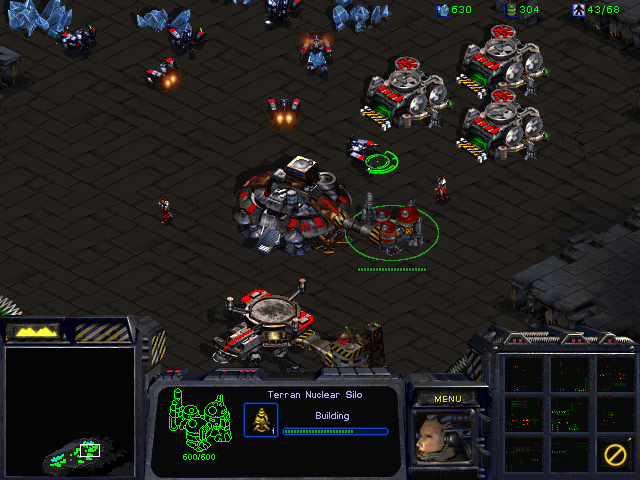
\includegraphics[scale=0.6]{media/starcraft-nuclear-silo.png}
	\caption{``Nuclear Sylow''.}
\end{figure}


Sylow's theorem is really huge for classifying groups;
in particular, the conditions $n_p \equiv 1 \pmod p$ and $n_p \mid m$
can often pin down the value of $n_p$ to just a few values.
Here are some results which follow from the Sylow theorems.
\begin{itemize}
	\ii A Sylow $p$-subgroup is normal if and only if $n_p = 1$.
	\ii Any group $G$ of order $pq$, where $p < q$ are primes,
	must have $n_q = 1$, since $n_q \equiv 1 \pmod q$ yet $n_q \mid p$.
	Thus $G$ has a normal subgroup of order $q$.
	\ii Since any abelian group has all subgroups normal,
	it follows that any abelian group has exactly one Sylow $p$-subgroup
	for every $p$ dividing its order.
	\ii If $p \neq q$, the intersection of a Sylow $p$-subgroup and a Sylow $q$-subgroup is just $\{1_G\}$.
	That's because the intersection of any two subgroups is also a subgroup,
	and Lagrange's theorem tells us that its order must divide both a power of $p$
	and a power of $q$; this can only happen if the subgroup is trivial.
\end{itemize}

Here's an example of another ``practical'' application.
\begin{proposition}[Triple product of primes]
	If $\left\lvert G \right\rvert = pqr$ is the product of distinct primes,
	then $G$ must have a normal Sylow subgroup.
\end{proposition}
\begin{proof}
	WLOG, assume $p<q<r$.  Notice that $n_p \equiv 1 \pmod p$, $n_p | qr$ and cyclically, and assume for contradiction that $n_p, n_q, n_r > 1$.
	
	Since $n_r | pq$, we have $n_r = pq$ since $n_r$ divides neither $p$ nor $q$ as $n_r \ge 1 + r > p,q$.  Also, $n_p \ge 1+p$ and $n_q \ge 1+q$.
	So we must have at least $1+p$ Sylow $p$-subgroups,
	at least $1+q$ Sylow $q$-subgroups, and at least $pq$ Sylow $r$-subgroups.

	But these groups are pretty exclusive.
	\begin{ques}
		Take the $n_p+n_q+n_r$ Sylow subgroups and consider two of them, 
		say $H_1$ and $H_2$.
		Show that $\left\lvert H_1 \cap H_2 \right\rvert = 1$
		as follows:
		check that $H_1 \cap H_2$ is a subgroup of both $H_1$ and $H_2$,
		and then use Lagrange's theorem.
	\end{ques}

	We claim that there are too many elements now.
	Indeed, if we count the non-identity elements contributed by these subgroups, we get
	\[ n_p(p-1) + n_q(q-1) + n_r(r-1)
		\ge (1+p)(p-1) + (1+q)(q-1) + pq(r-1) > pqr 
	\]
	which is more elements than $\left\lvert G \right\rvert$ has!
\end{proof}


\section{(Optional) Proving Sylow's theorem}
The proof of Sylow's theorem is somewhat involved,
and in fact many proofs exist.  I'll present one below here.
It makes extensive use of group actions,
so I want to recall the following facts first.
If $G$ acts on $X$, then
\begin{itemize}
	\ii The orbits of the action form a partition of $X$.
	\ii if $\OO$ is any orbit, then the orbit-Stabilizer theorem says that
	\[ \left\lvert \OO \right\rvert = \left\lvert G \right\rvert / \left\lvert \Stab_G(x) \right\rvert \]
	for any $x \in \OO$.
	\ii In particular: suppose in the above that $G$ is a group of order $p^t$.
	Then either $\left\lvert \OO \right\rvert = 1$ or $p$ divides $\left\lvert \OO \right\rvert$.
	In the case $\OO = \{x\}$, then by definition, $x$ is a \vocab{fixed point} of every element of $G$: we have $g \cdot x = x$ for every $x$.
\end{itemize}
Note that when I say $x$ is a fixed point, I mean it is fixed by \textbf{every} element of the group, i.e.\ the orbit really has size one. Hence that's a really strong condition.

\subsection*{Definitions}
\prototype{Conjugacy in $S_n$.}
In addition, I need the following definitions.
I've defined conjugacy of elements previously,
but I now need to define it for groups:
\begin{definition}
	Let $G$ be a group, and let $X$ denote the set of subgroups of $G$.
	Then \vocab{conjugation} is the action of $G$ on $X$ that sends
	\[ H \mapsto gHg\inv = \left\{ ghg\inv \mid h \in H \right\}. \]
	If $H$ and $K$ are subgroups of $G$ such that $H = gKg\inv$ for some $g \in G$
	(in other words, they are in the same orbit under this action),
	then we say they are \vocab{conjugate} subgroups.
\end{definition}

Because we somehow don't think of conjugate elements as
``that different'' (for example, in permutation groups),
the following shouldn't be surprising.
\begin{ques}
	Show that for any subgroup $H$ of a group $G$, the map $H \to gHg\inv$ by
	$h \mapsto ghg\inv$ is in fact an isomorphism.
	This implies that any two conjugate subgroups are isomorphic.
\end{ques}

\begin{definition}
	For any subgroup $H$ of $G$ the \vocab{normalizer} of $H$ is defined as
	\[ N_G(H) \defeq \left\{ g \in G \mid gHg\inv = H \right\}. \]
	In other words, it is the stabilizer of $H$ under the conjugation action.
\end{definition}

We are now ready to present the proof.

\subsection*{Step 1: Prove that a Sylow $p$-subgroup exists}
What follows is something like the probabilistic method.
By considering the set $X$ of ALL subsets of size $p^n$ at once, we can exploit the ``deep number theoretic fact'' that 
\[ \left\lvert X \right\rvert = \binom{p^n m}{p^n} \not\equiv 0 \pmod p. \]
(It's not actually deep: use Lucas' theorem.)

Here is the proof.
\begin{itemize}
	\ii Let $G$ act on $X$ by $g \cdot X \defeq \left\{ gx \mid x \in X \right\}$.
	\ii Take an orbit $\OO$ with size not divisible by $p$.
	(This is possible because of our deep number theoretic fact.
	Since $\left\lvert X \right\rvert$ is nonzero mod $p$ and the orbits partition $X$, the claimed orbit must exist. )
	\ii let $S \in \OO$, $H = \Stab_G(S)$. then $p^n$ divides $\left\lvert H \right\rvert$, by the orbit-Stabilizer theorem.
	\ii Consider a second action: let $H$ act on $S$ by 
	$h \cdot s \defeq hs$ (we know $hs \in S$ since $H = \Stab_G(S)$).
	\ii
	Observe that $\Stab_H(s) = \{1_H\}$.
	Then all orbits of the second action must have size $\left\lvert H \right\rvert$. Thus $\left\lvert H \right\rvert$ divides $\left\lvert S \right\rvert = p^n$.
	\ii This implies $\left\lvert H \right\rvert = p^n$, and we're done.
\end{itemize}


\subsection*{Step 2: Any two Sylow $p$-subgroups are conjugate}
Let $P$ be a Sylow $p$-subgroup (which exists by the previous step).
We now prove that for any $p$-group $Q$, $Q \subseteq gPg\inv$.
Note that if $Q$ is also a Sylow $p$-subgroup, then $Q = gPg\inv$ for size reasons;
this implies that any two Sylow subgroups are indeed conjugate.

\textbf{Let $Q$ act on the set of left cosets of $P$ by left multiplication.}
Note that
\begin{itemize}
	\ii $Q$ is a $p$-group, so any orbit has size divisible by $p$ unless it's $1$.
	\ii But the number of left cosets is $m$, which isn't divisible by $p$.
\end{itemize}
\textbf{Hence some coset $gP$ is a fixed point for every $q$}, meaning
$qgP = gP$ for all $q$.
Equivalently, $qg \in gP$ for all $q \in Q$, so $Q \subseteq gPg\inv$ as desired.


\subsection*{Step 3: Showing $n_p \equiv 1 \pmod p$}
Let $\mathcal S$ denote the set of all the Sylow $p$-subgroups.
Let $P \in \mathcal S$ be arbitrary.
\begin{ques}
	Why does $\left\lvert \mathcal S \right\rvert$ equal $n_p$?
	(In other words, are you awake?)
\end{ques}
Now we can proceed with the proof.
Let $P$ act on $\mathcal S$ by conjugation.
Then:
\begin{itemize}
	\ii Because $P$ is a $p$-group, $n_p \pmod p$ is the number of fixed points
	of this action.
	Now we claim $P$ is the only fixed point of this action.
	\ii Let $Q$ be any other fixed point, meaning $xQx\inv = Q$ for any $x \in G$.
	\ii Define the normalizer $N_G(Q) = \left\{ g \in G \mid gQg\inv = Q \right\}$.  It contains both $P$ and $Q$.
	\ii Now for the crazy part: apply Step 2 to $N_G(Q)$.
	Since $P$ and $Q$ are Sylow $p$-subgroups of it, they must be conjugate.
	\ii Hence $P=Q$, as desired.
\end{itemize}

\subsection*{Step 4: $n_p$ divides $m$}
Since $n_p \equiv 1 \pmod p$, it suffices to show $n_p$ divides $\left\lvert G \right\rvert$.
Let $G$ act on the set of all Sylow $p$-groups by conjugation.
Step 2 says this action has only one orbit, so the Orbit-Stabilizer theorem
implies $n_p$ divides $\left\lvert G \right\rvert$.


\section{(Optional) Simple groups and Jordan-H\"older}
\prototype{Decomposition of $\Zc{12}$ is $1 \normalin \Zc 2 \normalin \Zc 4 \normalin \Zc{12}$.}
% Fortunately, there is at least a way to ``break down'' $G$.
Just like every integer breaks down as the product of primes,
we can try to break every group down as a product of ``basic'' groups.
Armed with our idea of quotient groups, the right notion is this.

\begin{definition}
	A \vocab{simple group} is a group with no normal subgroups
	other than itself and the trivial group.
\end{definition}
\begin{ques}
	For which $n$ is $\Zc n$ simple? (Hint: remember that $\Zc n$ is abelian.)
\end{ques}

\begin{figure}[ht]
	\centering
	\snsd[height=7cm]{my-world-symmetric-group.png}
	\caption{The group $S_n$ is simple when $n=2$. Also, Google ``solvable groups''.}
\end{figure}


Then we can try to define what it means to ``break down a group''.
\begin{definition}
	A \vocab{composition series} of a group $G$ is a sequence of subgroups
	$H_0$, $H_1$, \dots, $H_n$ such that
	\[ \{1\} = H_0 \normalin H_1 \normalin H_2 \normalin \dots \normalin H_n
		\normalin G \]
	of maximal length (i.e.\ $n$ is as large as possible,
	but all $H_i$ are of course distinct).
	The \vocab{composition factors} are the groups
	$H_1/H_0$, $H_2/H_1$, \dots, $H_n/H_{n-1}$.
\end{definition}
You can show that the ``maximality'' condition implies that the composition factors are all simple groups.

Let's say two composition series are equivalent if they have the same composition factors (up to permutation); in particular they have the same length.
Then it turns out that the following theorem \emph{is} true.
\begin{theorem}
	[Jordan-H\"older]
	Every finite group $G$ admits a unique composition series up to equivalence.
\end{theorem}

\begin{example}
	[Fundamental theorem of arithmetic when $n=12$]
	Let's consider the group $\Zc{12}$.
	It's not hard to check that the possible composition series are
	\begin{align*}
		\{1\} \normalin \Zc2 \normalin \Zc4 \normalin \Zc{12}
		& \text{ with factors $\Zc2$, $\Zc2$, $\Zc3$} \\
		\{1\} \normalin \Zc2 \normalin \Zc6 \normalin \Zc{12}
		& \text{ with factors $\Zc2$, $\Zc3$, $\Zc2$} \\
		\{1\} \normalin \Zc3 \normalin \Zc6 \normalin \Zc{12}
		& \text{ with factors $\Zc3$, $\Zc2$, $\Zc2$}.
	\end{align*}
	These correspond to the factorization $12 = 2^2 \cdot 3$.
\end{example}

This suggests that classifying all finite simple groups would be great progress, since every finite group is somehow a ``product'' of simple groups;
the only issue is that there are multiple ways of building a group from constituents.

Amazingly, we actually \emph{have} a full list of simple groups,
but the list is really bizarre.
Every finite simple group falls in one of the following categories:
\begin{itemize}
	\ii $\Zc p$ for $p$ a prime,
	\ii For $n \ge 5$, the subgroup of $S_n$ consisting of ``even'' permutations.
	\ii A simple group of Lie type (which I won't explain), and
	\ii Twenty-six ``sporadic'' groups which do not fit into any nice family.
\end{itemize}
The two largest of the sporadic groups have cute names.
The \vocab{baby monster group} has order 
\[ 2^{41} \cdot 3^{13} \cdot 5^6 \cdot 7^2 \cdot 11 \cdot 13 \cdot 17
	\cdot 19 \cdot 23 \cdot 31 \cdot 47 \approx 4 \cdot 10^{33} \]
and the \vocab{monster group} (also ``\vocab{friendly giant}'') has order
\[ 
	2^{46} \cdot 3^{20} \cdot 5^9 \cdot 7^6 \cdot 11^2 \cdot 13^3
	\cdot 17 \cdot 19 \cdot 23 \cdot 29 \cdot 31 \cdot 41 \cdot 47
	\cdot 59 \cdot 71 \approx 8 \cdot 10^{53}. \]
It contains twenty of the sporadic groups as subquotients (including itself),
and these twenty groups are called the ``\vocab{happy family}''.

\begin{figure}[ht]
	\centering
	\includegraphics[width=0.5\textwidth]{media/monster.jpg}
	\caption{On the topic of monsters\dots}
\end{figure}

Math is weird.

\begin{ques}
	Show that ``finite simple group of order $2$'' is redundant
	in the sense that any group of order $2$ is both finite and simple.
\end{ques}

\section\problemhead


\begin{sproblem}
	[Cauchy's theorem]
	Let $G$ be a group and let $p$ be a prime dividing $\left\lvert G \right\rvert$.
	Prove\footnote{
		Cauchy's theorem can be proved without the Sylow theorems,
		and in fact can often be used to give alternate proofs of Sylow.}
	that $G$ has an element of order $p$.
	\label{thm:cauchy_group}
\end{sproblem}

\begin{problem}
	Let $G$ be a finite simple group.
	Show that $\left\lvert G \right\rvert \neq 56$.
	\begin{hint}
		Count Sylow $8$ and $7$ groups and let them intersect.
	\end{hint}
	\begin{sol}
		If not, there exists eight Sylow $7$-groups and seven Sylow $8$-groups
		(since $n_7 \equiv 1 \pmod 7$, $n_8 \mid 7$, and $n_7, n_8 > 1$).
		But no two of thees $8+7=15$ groups can intersect at an element other than $1_G$,
		which is clearly absurd.
	\end{sol}
\end{problem}

\begin{problem}
	[Engel's PSS?]
	\gim
	Consider the set of all words consisting of the letters $a$ and $b$.
	Given such a word, we can change the word either by inserting a word of the form $www$,
	where $w$ is a word, anywhere in the given word, or by deleting such a sequence from the word.
	Can we turn the word $ab$ into the word $ba$?
	% http://www.artofproblemsolving.com/Forum/viewtopic.php?f=780&t=456603&p=2572053
	% lol Alex Zhu op
	\begin{hint}
		Construct a non-abelian group such that all elements have order three.
	\end{hint}
	\begin{sol}
		One example is upper triangular matrices with entries in mod $3$.
	\end{sol}
\end{problem}

\begin{problem}
	\yod
	Let $p$ be a prime.
	Show that the only simple group with order $p^n$
	(for some positive integer $n$)
	is the cyclic group $\Zc p$.

	% class equation
	\begin{hint}
		First, if $G$ abelian it's trivial.
		Otherwise, let $Z(G)$ be the center of the group,
		which is always a normal subgroup of $G$.
		Do a mod $p$ argument via conjugation (or use the class equation).
	\end{hint}
	\begin{sol}
		Let $G$ be said group.
		If $G$ is abelian then all subgroups are normal,
		and since $G$ is simple, $G$ can't have any subgroups at all.
		We can clearly find an element of order $p$, hence $G$ has a subgroup
		of order $p$, which can only happen if $n=1$, $G \cong \Zc p$.

		Thus it suffices to show $G$ can't be abelian.
		For this, we can use the class equation, but let's avoid that and do it directly:

		Assume not and let $Z(G) = \{ g \in G \mid xg = gx \; \forall x \in G \}$
		be the center of the group.
		Since $Z(G)$ is normal in $G$, and $G$ is simple, we see $Z(G) = \{1_G\}$.
		But then let $G$ act on itself by conjugation: $g \cdot x = gxg\inv$.
		This breaks $G$ into a bunch of orbits $\OO_0 = \{1_G\}$, $\OO_1$, $\OO_2$, \dots,
		and since $1_G$ is the only fixed point by definition, all other orbits
		have size greater than $1$.
		The Orbit-stabilizer theorem says that each orbit now has size dividing $p^n$,
		so they must all have size zero mod $p$.

		But then summing across all orbits (which partition $G$),
		we obtain $\left\lvert G \right\rvert \equiv 1 \pmod p$,
		which is a contradiction.
	\end{sol}
\end{problem}
